\chapter{Preprocesamientos}

En este capítulo se describirán distintos tipos de preprocesamientos que pueden ser aplicados a los datos. Posteriormente, se procederá a realizar experimentos utilizando cada uno de estos preprocesamientos en combinación con SVM, evaluando si hay alguna mejora en los resultados que fueron expuestos en el capítulo anterior. Se utilizarán las implementaciones provistas por el módulo \textit{preprocessing} de SKLearn \cite{sklearn_api}, cuyos detalles pueden consultarse en la documentación de SKLearn\footnote{ \url{https://scikit-learn.org/stable/modules/preprocessing.html} }. 

\section { Estandarización }

En primer lugar, se consideraron distintas técnicas básicas que consisten en modificar la media y escalar la varianza de los datos. \cite{han2012mining}

\begin{itemize}
\item \textbf{MaxAbsScaler}: Escalar cada atributo por separado al rango $[-1,1]$. Para cada columna $c$, se dividen todos los elementos de esa columna por su máximo valor absoluto:

\begin{center}
$ c := \frac{c}{max(abs(c))} $
\end{center}

\item \textbf{MinMaxScaler}: Escalar cada atributo por separado al rango $[0,1]$. Para cada columna $c$, se aplica la siguiente transformación \cite{han2012mining}:

\begin{center}
$ c := \frac{ c - min(c) } { max(c) - min(c) }$
\end{center}

\item \textbf{StandardScaler}: Estandarizar cada atributo, restándole su media y escalando a varianza unitaria.

\begin{center}
$ c := \frac{ c - mean(c) } { stdev(c) }$
\end{center}

\item \textbf{RobustScaler}: Estandarizar cada atributo usando métricas robustas a outliers, restando la mediana y escalando los datos de acuerdo al rango intercuartil.

\end{itemize}

\section { Transformaciones no lineales y discretización}

En esta sección se enumeran distintas técnicas que modifican la distribución de probabilidad subyacente de cada atributo:

\begin{itemize}

\item \textbf{PowerTransformer}: Aplica una transformación paramétrica, monotónica que transforma cada atributo para que tenga una distribución de probabilidad más Gaussiana. La transformación utilizada es  Yeo-Johnson \cite{yeo}. Un escalado estándar (StandardScaler) es aplicado previamente a los datos.

\item \textbf {QuantileTransformer}: Transformar cada atributo por separado, obteniendo valores entre 0 y 1. Una primera opción es mapear los datos a una distribución uniforme, una segunda opción es mapear los datos a una distribución normal \cite{KRZYSZTOFOWICZ1997286}. Un parámetro de esta transformación es el número de cuantiles computado para realizar la transformación.

\item \textbf {Binning}: Discretizar cada atributo por separado, distribuyendo sus valores en $k$ cubetas (bins) \cite{han2012mining}. Distintos criterios pueden seguirse para decidir cómo se distribuyen los datos en cada cubeta:
\begin{itemize}
\item \textbf{Uniforme}: Usar cubetas de tamaño constante. Es decir, dividir el rango de valores del atributo en $k$ intervalos del mismo tamaño; y reemplazar cada valor por el índice de su intervalo.
\item \textbf{Quantile}: Colocar la misma cantidad de elementos en cada cubeta.
\item \textbf{Kmeans}: Definir cada cubeta basado en un algoritmo de clústering k-means. 
\end{itemize}
\end{itemize}


Es importante remarcar que para todos los preprocesamientos discutidos hasta el momento, se estimarán los parámetros de la transformación usando únicamente los datos de entrenamiento. Por ejemplo, los límites de los bins son calculados sobre los datos de entrenamiento y estos mismos límites se utilizarán para discretizar los datos de test. Análogamente, a la hora de realizar un escalado estándar por ejemplo, tanto a los datos de entrenamiento como a los de test se les resta la media del dataset de entrenamiento y se les divide por la varianza del detaset de entrenamiento.

\section { Preprocesamientos en SVM Lineal }

Se aplicaron los preprocesamientos descriptos en las secciones anteriores a los datos, antes de utilizar SVM Lineal. En los siguientes experimentos, se considera como baseline la performance reportada en la última sección del capítulo anterior, obtenida aplicando únicamente StandardScaler antes de entrenar y testear. 

\begin{itemize}

\item Los resultados de aplicar estandarización pueden ser observados en \ref{fig:svml_estandarizacion}. De este experimento se desprende que StandardScaler es la mejor opción, dado que es la única opción que se encuentra consistentemente entre los preprocesamientos con mejor performance.

\item Los resultados de aplicar QuantileTransformer se pueden observar en \ref{fig:svml_quantiles}. Se exploraron ambas variantes: mapear la distribución de cada atributo a una distribución normal, y a una distribución uniforme. Para cada una de estas configuraciones, se analizó el R-AUPRC en función del número de cuantiles utilizado en el transformador. Podemos observar que todas las combinaciones de parámetros exploradas efectivamente incrementan la performance respecto al baseline; aunque el número de cuantiles óptimo es dependiente de los datos.

\item Los resultados de aplicar binning, seguido de un escalado estándar, se pueden observar en \ref{fig:svml_binning}. Se exploraron las tres estrategias anteriormente mencionadas (Uniform, Quantile y Kmeans), estudiando la evolución del R-AUPRC en función del número de cubetas. Se puede apreciar que la estrategia Quantile es consistentemente la mejor opción. Nótese que la estrategia KMeans es computacionalmente impracticable para grandes cantidades de cubetas.

\item Las curvas de precision-recall de los preprocesamientos que tuvieron mejor desempeño en los experimentos anteriores, junto con la correspondiente a PowerTransformer (que no requiere parámetros), son comparadas en la figura \ref{fig:svml_final_comparison}. De esta comparación final se desprende que el preprocesamiento óptimo para SVM Lineal es binning, seguido de un escalado estándar. Al final de este capítulo se especula sobre los motivos por los cuales binning produce tales mejoras.
\end{itemize}


\begin{figure}[h!]
\begin{tabular}{cccc}
  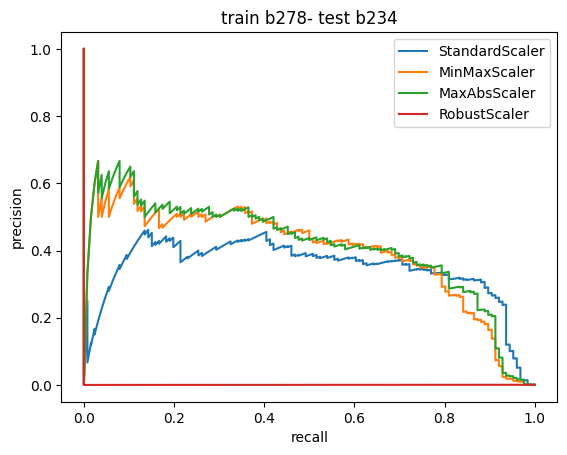
\includegraphics[width=0.25\textwidth]{Kap4/Figure_1.png}  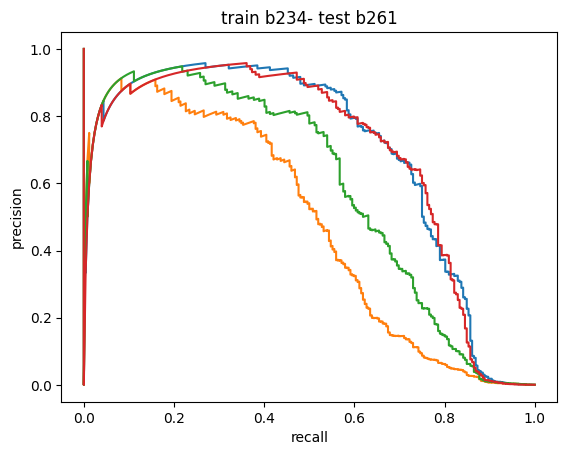
\includegraphics[width=0.25\textwidth]{Kap4/Figure_2.png} 
  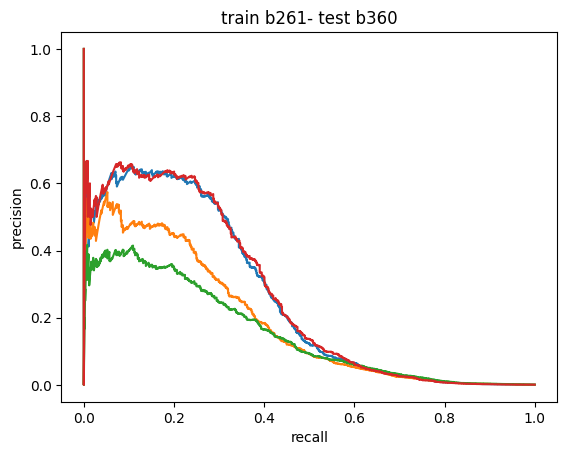
\includegraphics[width=0.25\textwidth]{Kap4/Figure_3.png}  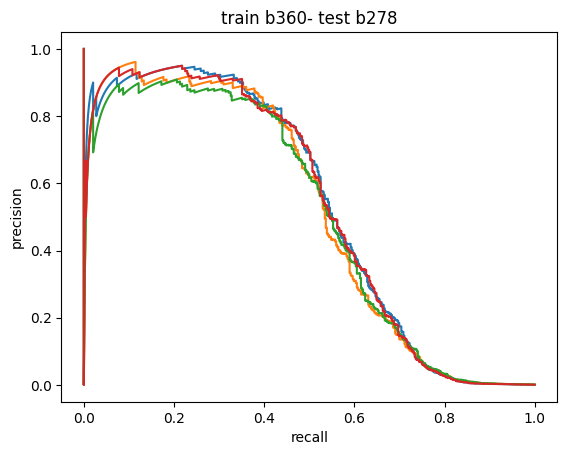
\includegraphics[width=0.25\textwidth]{Kap4/Figure_4.png} 
\end{tabular}
\caption{Estandarización en SVM Lineal.}
\label{fig:svml_estandarizacion}
\end{figure}

\begin{figure}[h!]
\begin{tabular}{cccc}
  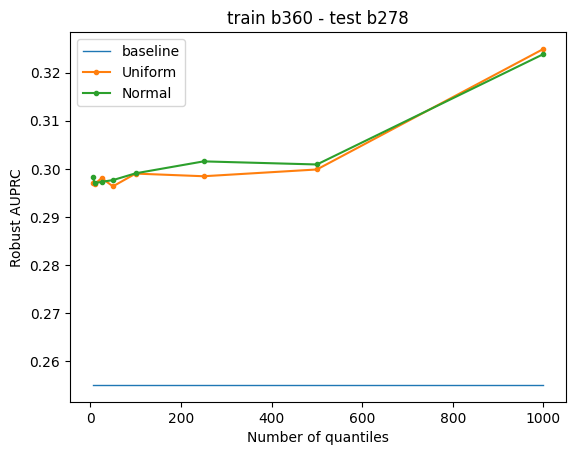
\includegraphics[width=0.25\textwidth]{Kap4/Figure_5.png}  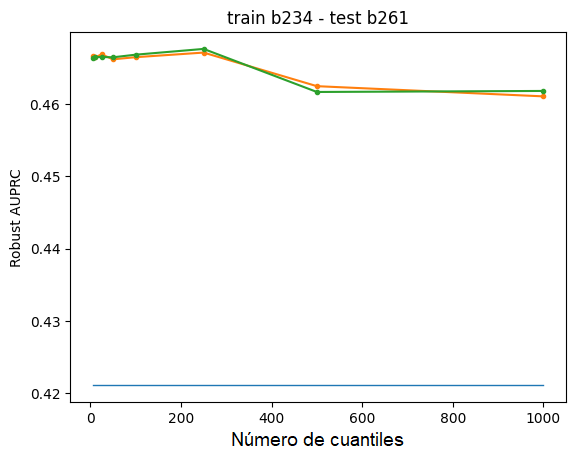
\includegraphics[width=0.25\textwidth]{Kap4/Figure_6.png}
  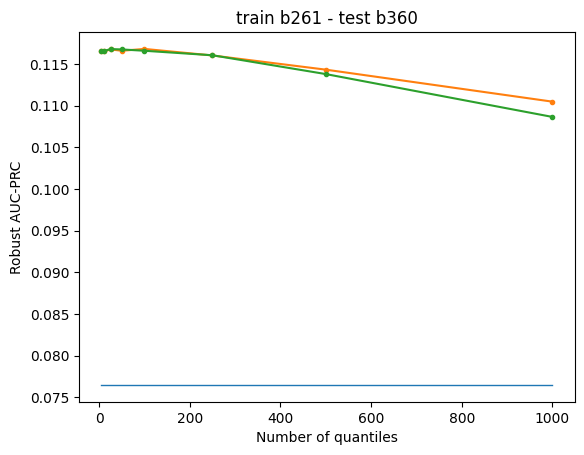
\includegraphics[width=0.25\textwidth]{Kap4/Figure_7.png}  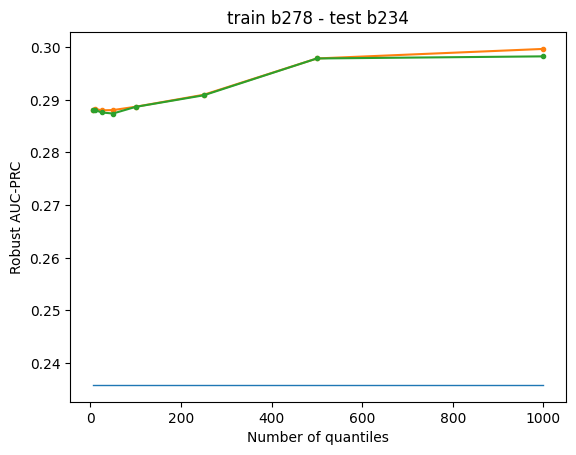
\includegraphics[width=0.25\textwidth]{Kap4/Figure_8.png} 
\end{tabular}
\caption{QuantileTransformer en SVM Lineal}
\label{fig:svml_quantiles}
\end{figure}

\begin{figure}[h!]
\begin{tabular}{cccc}
  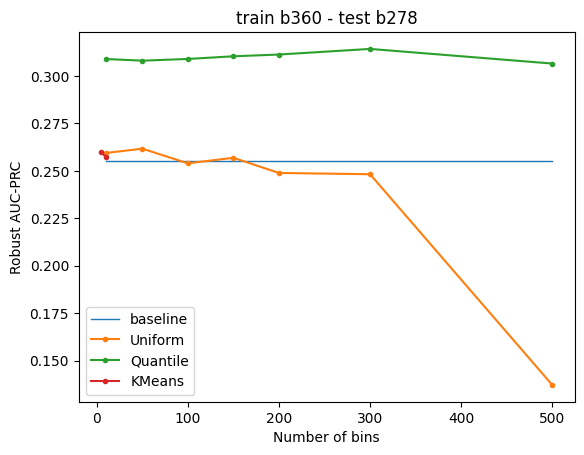
\includegraphics[width=0.25\textwidth]{Kap4/Figure_9.png}  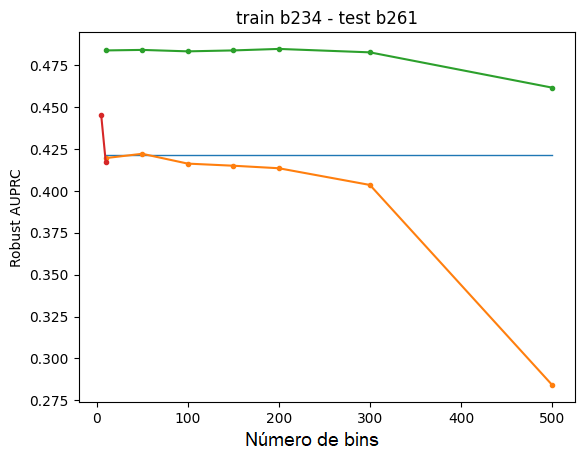
\includegraphics[width=0.25\textwidth]{Kap4/Figure_10.png}
  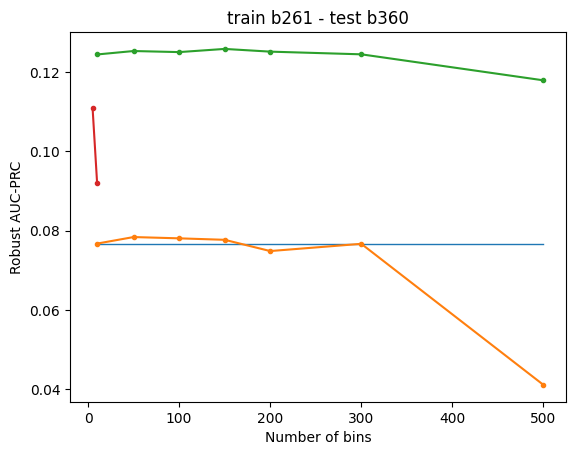
\includegraphics[width=0.25\textwidth]{Kap4/Figure_11.png} 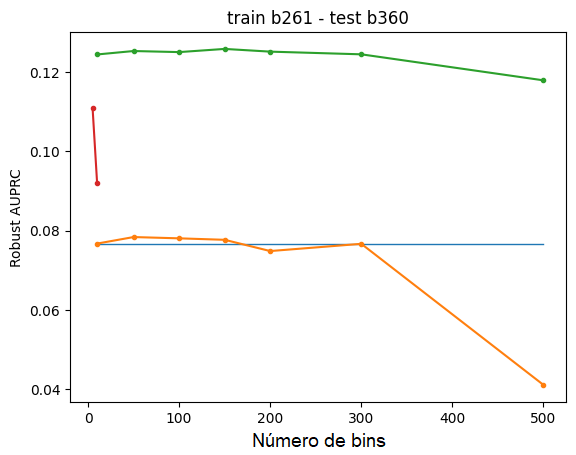
\includegraphics[width=0.25\textwidth]{Kap4/Figure_12.png} 
\end{tabular}
\caption{Binning en SVM Lineal}
\label{fig:svml_binning}
\end{figure}

\begin{figure}[h!]
\begin{tabular}{cccc}
  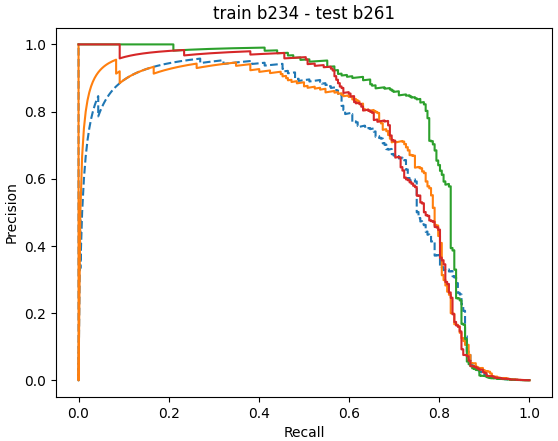
\includegraphics[width=0.25\textwidth]{Kap4/Figure_13.png}  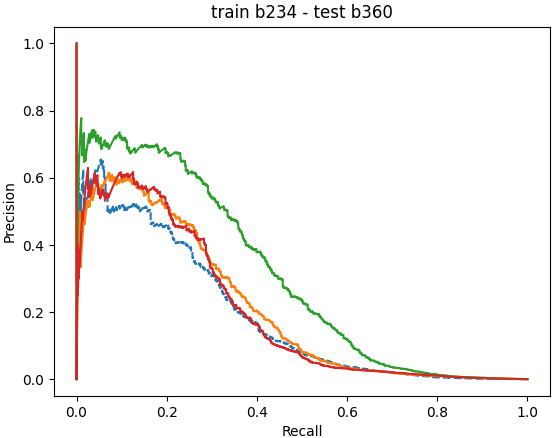
\includegraphics[width=0.25\textwidth]{Kap4/Figure_14.png}
  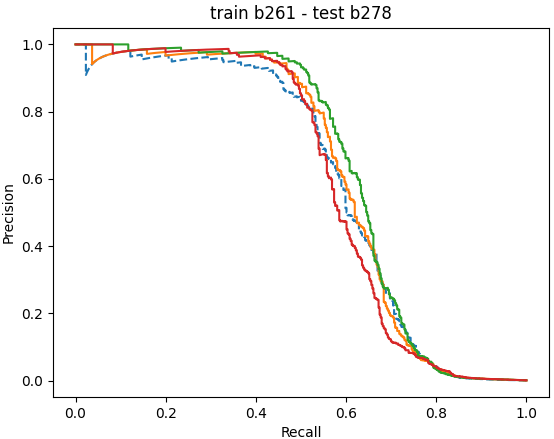
\includegraphics[width=0.25\textwidth]{Kap4/Figure_15.png}  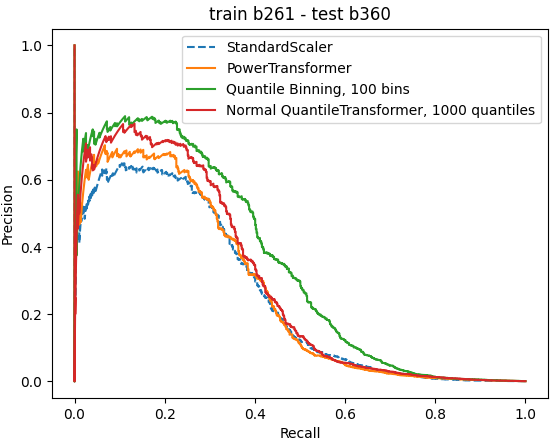
\includegraphics[width=0.25\textwidth]{Kap4/Figure_16.png} \\

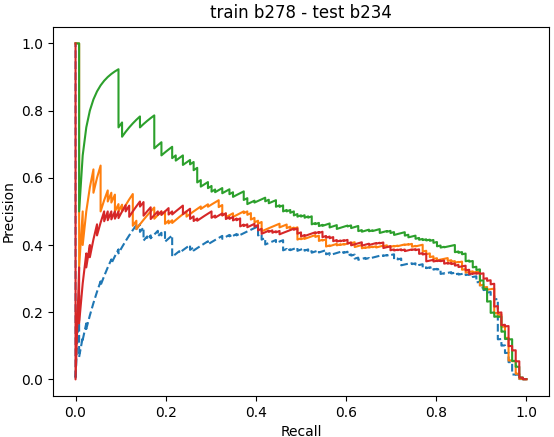
\includegraphics[width=0.25\textwidth]{Kap4/Figure_17.png}  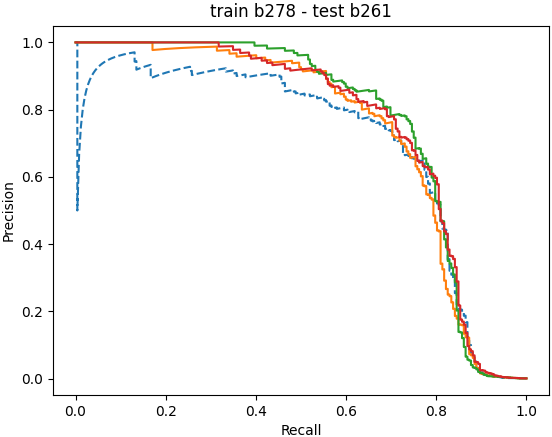
\includegraphics[width=0.25\textwidth]{Kap4/Figure_18.png} 
 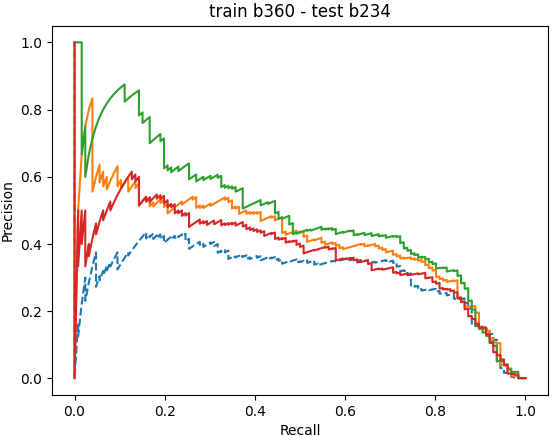
\includegraphics[width=0.25\textwidth]{Kap4/Figure_19.png}  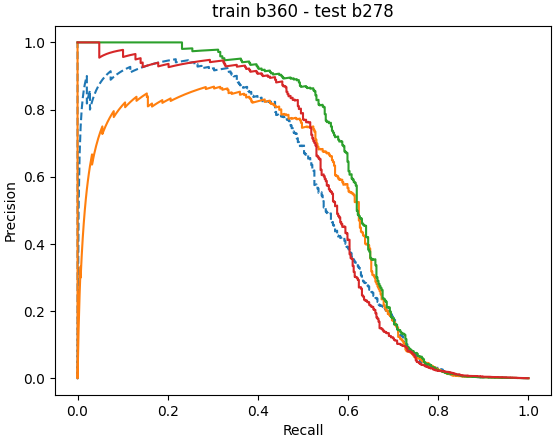
\includegraphics[width=0.25\textwidth]{Kap4/Figure_20.png} 
\end{tabular}
\caption{Comparación de los mejores preprocesamientos, SVM Lineal}
\label{fig:svml_final_comparison}
\end{figure}



\section{Preprocesamientos en SVM RBF}

Se procedió a realizar los mismos experimentos utilizando SVM con kernel RBF:

\begin{itemize}
\item Los resultados de aplicar estandarización pueden ser observados en \ref{fig:svmk_estandarizacion}. Nuevamente, StandardScaler parece ser la mejor opción, estando consistentemente entre los que mejor funcionan. El escalado robusto, si bien produce mejores resultados en ciertos tiles, ocasiona una pérdida significativa de performance en otros.

\item Los resultados de aplicar QuantileTransformer se pueden observar en \ref{fig:svmk_quantiles}. A diferencia de en SVM-Lineal, la performance oscila considerablemente dependiendo del número de cuantiles, y es difícil encontrar una asignación de parámetros para este método que sea óptima para todos los tiles. Más aún, aplicar este preprocesamiento implica una pérdida de performance respecto al baseline algunas de las combinaciones testeadas, por lo cuál se descarta su aplicación en el resto de este trabajo.

\item Los resultados de aplicar binning, seguido de un escalado estándar, se pueden observar en \ref{fig:svmk_binning}. Los resultados son consistentes a los observados en SVM Lineal: La estrategia Quantile es consistentemente superior a las otras estrategias, y dependiendo del número de bins escogido mejora la performance respecto al baseline. 

\item Las curvas de precision-recall de los preprocesamientos que tuvieron mejor desempeño en los experimentos anteriores, junto con la correspondiente a PowerTransformer (que no requiere parámetros), son comparadas en la figura \ref{fig:svmk_final_comparison}. De esta comparación final se desprende que el preprocesamiento óptimo para SVM RBF es Binning, aunque la mejora es mucho más modesta que la obtenida en SVM Lineal.
\end{itemize}


\begin{figure}[h!]
\begin{tabular}{cccc}
  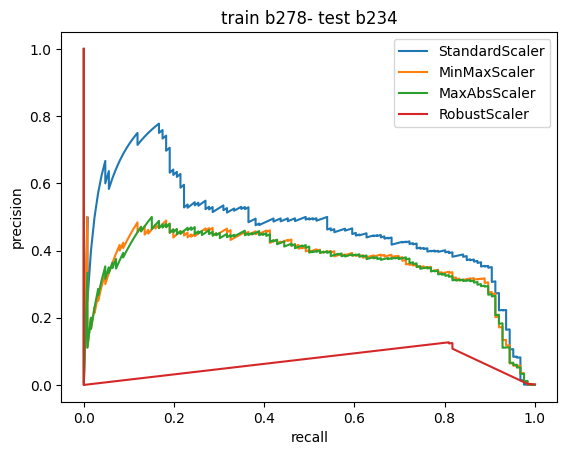
\includegraphics[width=0.25\textwidth]{Kap4/kFigure_1.png}  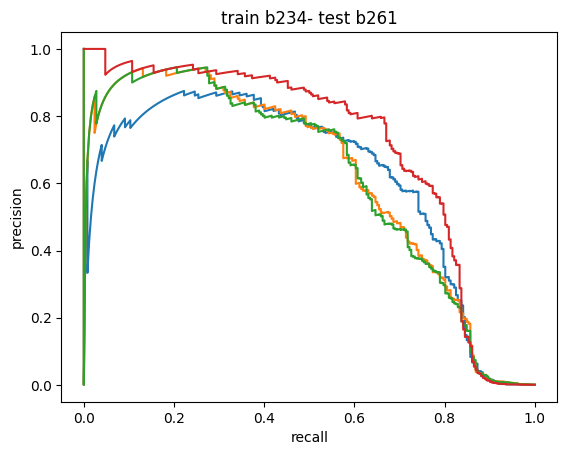
\includegraphics[width=0.25\textwidth]{Kap4/kFigure_2.png}
  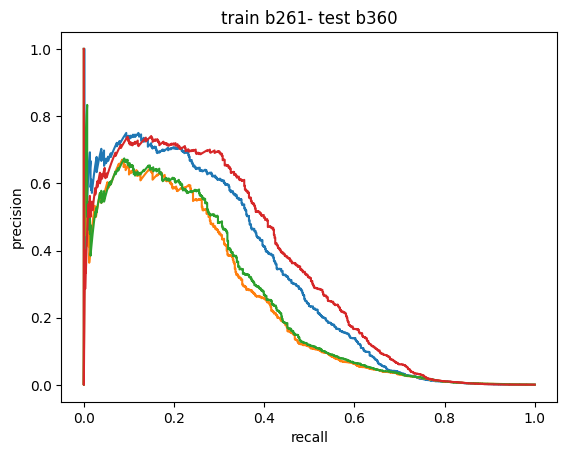
\includegraphics[width=0.25\textwidth]{Kap4/kFigure_3.png}  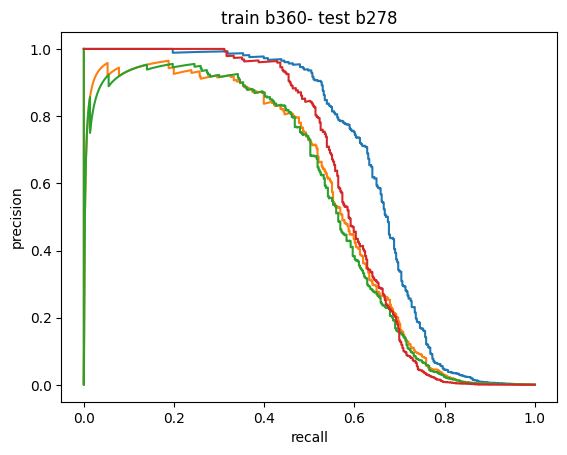
\includegraphics[width=0.25\textwidth]{Kap4/kFigure_4.png} 
\end{tabular}
\caption{Estandarización en SVM RBF}
\label{fig:svmk_estandarizacion}
\end{figure}

\begin{figure}[h!]
\begin{tabular}{cccc}
  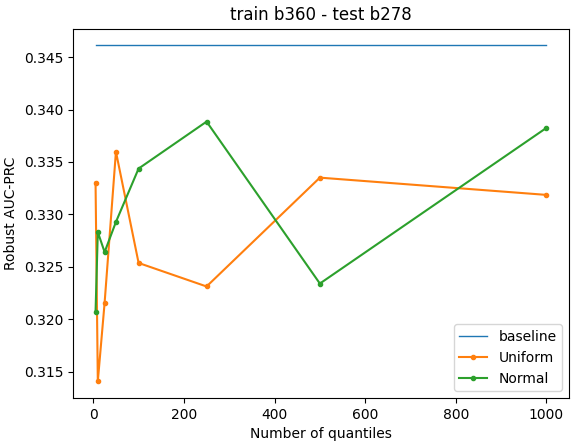
\includegraphics[width=0.25\textwidth]{Kap4/kFigure_5.png}  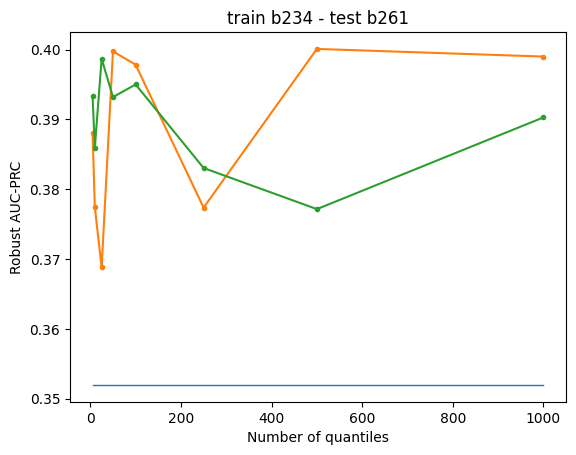
\includegraphics[width=0.25\textwidth]{Kap4/kFigure_6.png}
  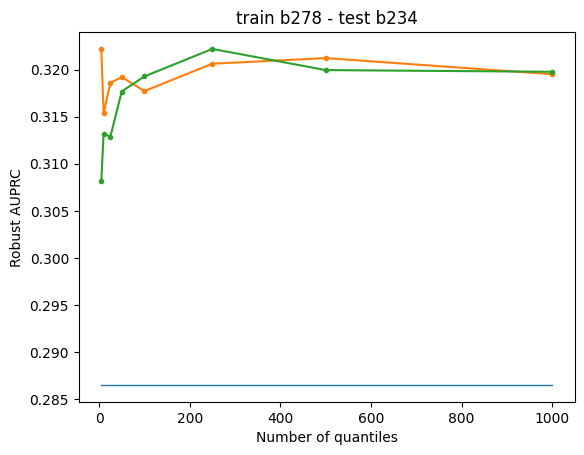
\includegraphics[width=0.25\textwidth]{Kap4/kFigure_8.png}  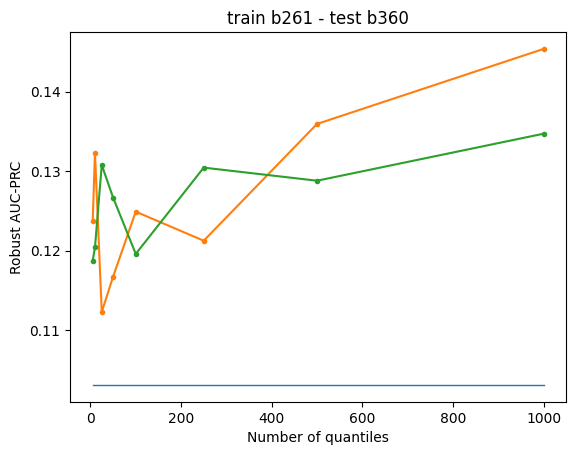
\includegraphics[width=0.25\textwidth]{Kap4/kFigure_7.png} 
\end{tabular}
\caption{QuantileTransformer en SVM RBF}
\label{fig:svmk_quantiles}
\end{figure}

\begin{figure}[h!]
\begin{tabular}{cccc}
  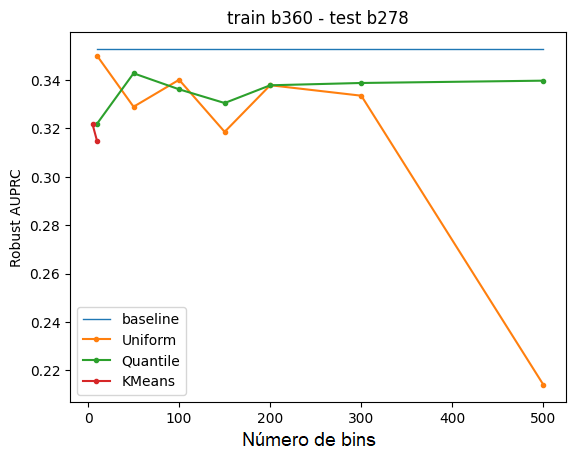
\includegraphics[width=0.25\textwidth]{Kap4/kFigure_9.png} 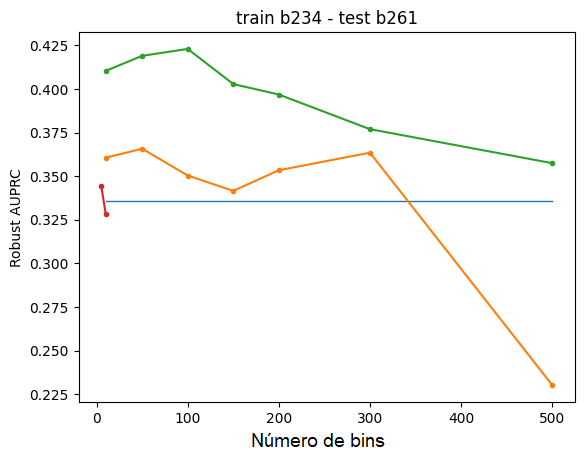
\includegraphics[width=0.25\textwidth]{Kap4/kFigure_10.png}
  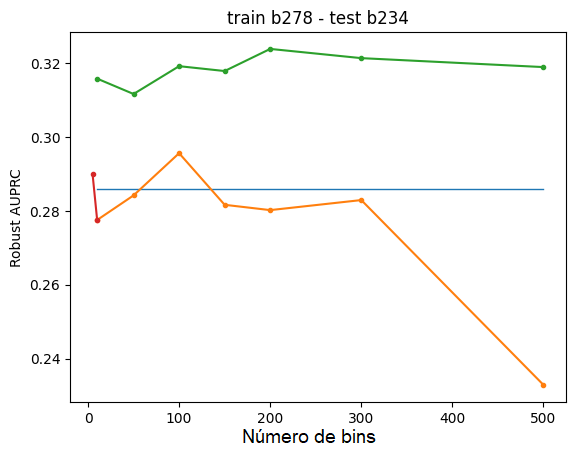
\includegraphics[width=0.25\textwidth]{Kap4/kFigure_11.png} 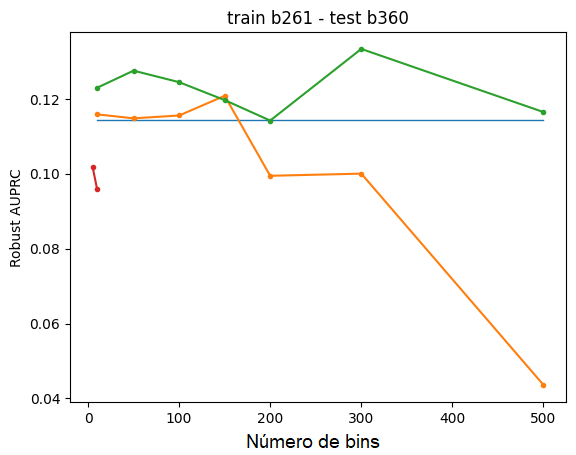
\includegraphics[width=0.25\textwidth]{Kap4/kFigure_12.png} 
\end{tabular}
\caption{Binning en SVM RBF}
\label{fig:svmk_binning}
\end{figure}

\begin{figure}[h!]
\begin{tabular}{cccc}
  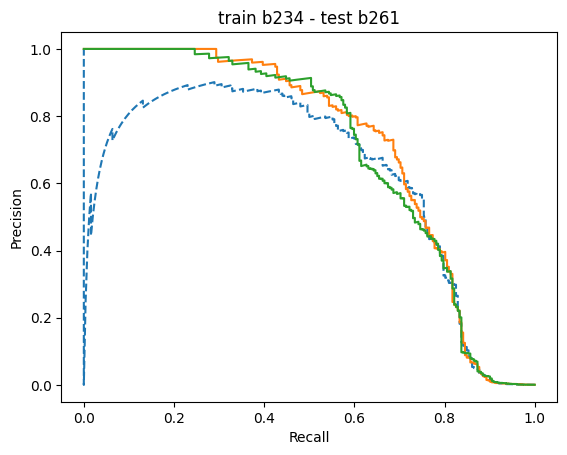
\includegraphics[width=0.25\textwidth]{Kap4/kFigure_13.png}  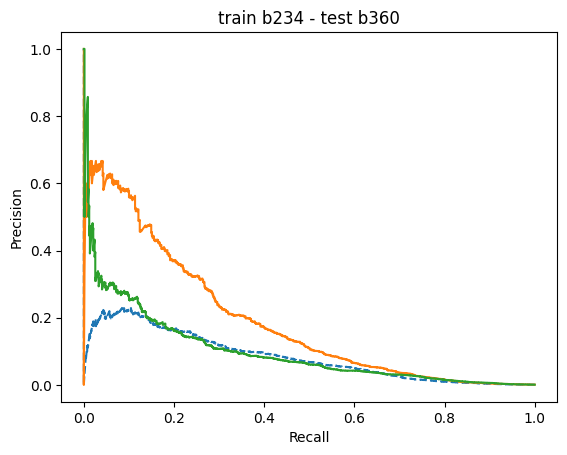
\includegraphics[width=0.25\textwidth]{Kap4/kFigure_14.png} 
  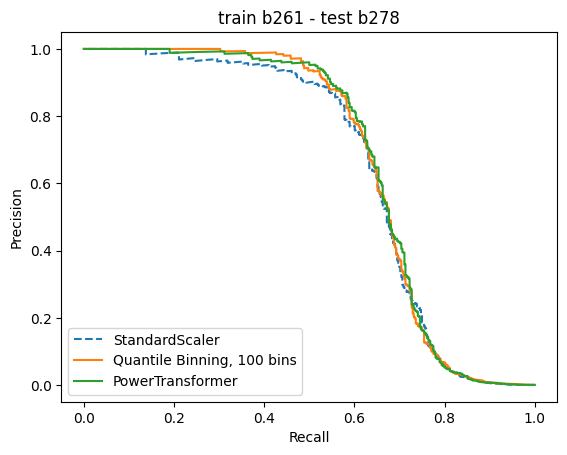
\includegraphics[width=0.25\textwidth]{Kap4/kFigure_15.png}  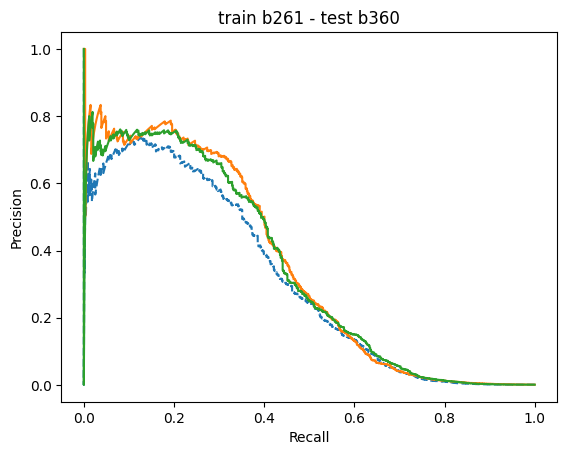
\includegraphics[width=0.25\textwidth]{Kap4/kFigure_16.png} \\
	  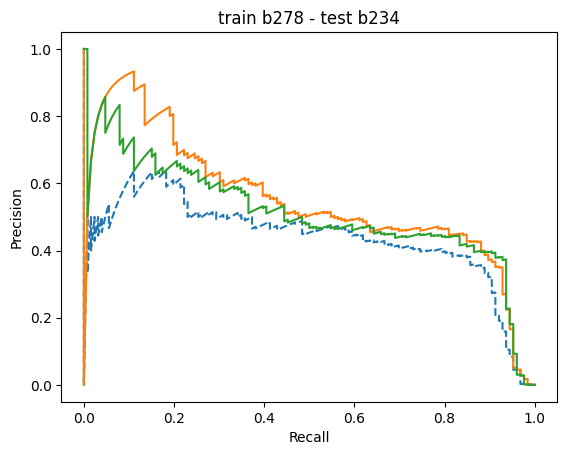
\includegraphics[width=0.25\textwidth]{Kap4/kFigure_17.png}  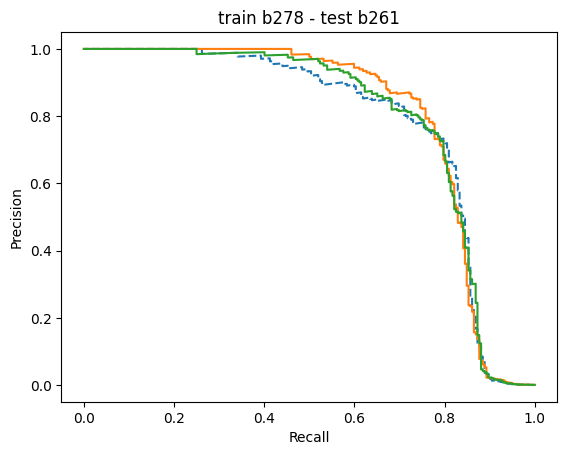
\includegraphics[width=0.25\textwidth]{Kap4/kFigure_18.png} 
		  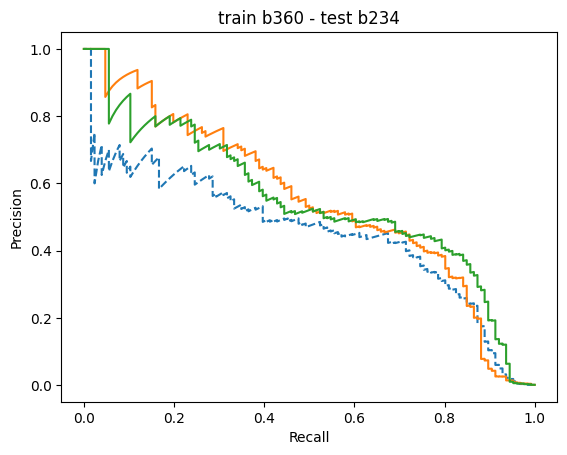
\includegraphics[width=0.25\textwidth]{Kap4/kFigure_19.png}  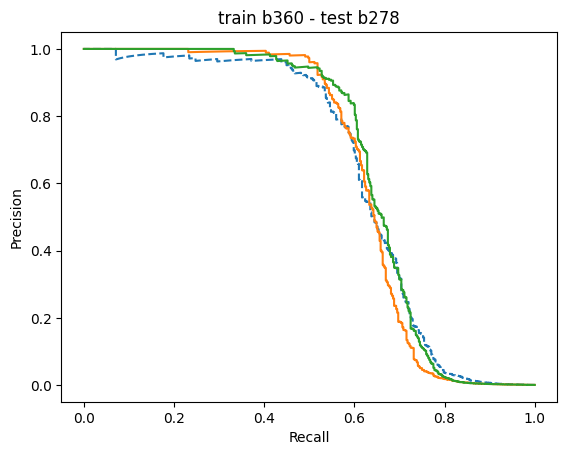
\includegraphics[width=0.25\textwidth]{Kap4/kFigure_20.png}
\end{tabular}
\caption{Comparación de los mejores preprocesamientos, SVM RBF}
\label{fig:svmk_final_comparison}
\end{figure}

\section{Análisis de resultados}

Se exploró una amplia variedad de preprocesamientos a ser aplicados a los datos. Aquellas técnicas que transforman la distribución de probabilidad de cada atributo a una normal o uniforme fueron las que mostraron un mayor beneficio, siendo Binning el preprocesamiento escogido para el resto de este trabajo. \\

Hay distintos motivos por los cuales binning quantile puede estar mejorando consistentemente la performance de SVM:

\begin{itemize}
\item Errores de medición: Se reduce el efecto de errores menores de observación. Es decir, se aplica un efecto de suavizado local (local smoothing) sobre los datos. Esto es razonable para datasets astronómicos, donde los instrumentos de medición que generan los datos siempre tendrán un error inherente.
\item Manejo de outliers: Valores extremos son asignados a las cubetas de los extremos, evitando que tengan un efecto significativo sobre los parámetros del modelo.
\item Binning tiene una cierta similitud a la forma en que los árboles de decisión funcionan: dividir una variable continua en subintervalos, eligiendo ciertos puntos de corte; y tomar decisiones dependiendo de en qué subintervalo un cierto valor está. Es posible que para nuestros datos, ciertas variables tengan un efecto particular sobre la clase objetivo a un threshold específico; y binning ayude a SVM a \textit{entender} esto con mayor facilidad, concentrándose en interacciones de alto orden entre las variables.
\item La distribución de probabilidad subyacente de cada atributo será convertida a una distribución uniforme.
\end{itemize} 

Claramente, la potencial pérdida de información asociada a discretizar los datos no perjudica a nuestro modelo. Nótese que se aplica un escalado estándar luego de Binning, dado que Binning en su forma pura mapearía cada valor a $[0,NBINS)$; y SVM funciona mejor con valores pequeños alrededor de cero. \\

\section{Reoptimización de hiperparámetros}

Luego de definir el preprocesamiento óptimo de cada método (Quantile 100-Binning + StandardScaler), se procedió a reoptimizar los hiperparámetros tal y como se describió en el capítulo 3, esta vez incluyendo los preprocesamientos. Los nuevos parámetros óptimos fueron: 

\begin{itemize}
\item \textbf{SVM-Lineal:} $C=10$ y 150 bins.
\item \textbf{SVM-RBF:} $C=10^4$, $\gamma = 10^{-4}$, 100 bins.
\end{itemize}  

Notemos que el parámetro C ahora es dos órdenes de magnitud mayor en SVM-Lineal, y un orden de magnitud menor en SVM-RBF. El R-AUPRC en cross-validation obtenido para cada clasificador puede observarse en la figura \ref{fig:reopt_param}. \\

\begin{figure}[h!]
\begin{tabular}{cc}
  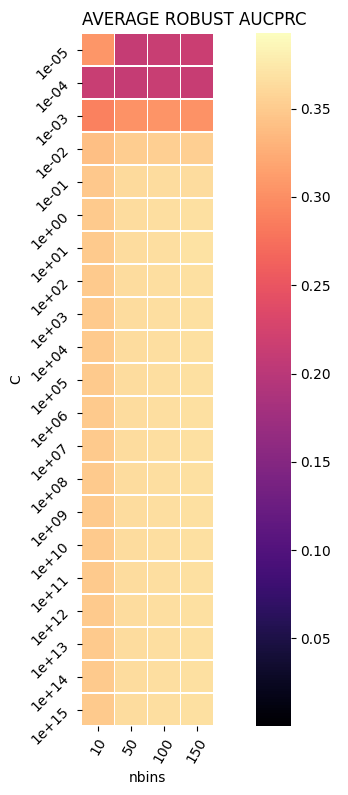
\includegraphics[width=0.29\textwidth]{Kap4/reoptl.png} &   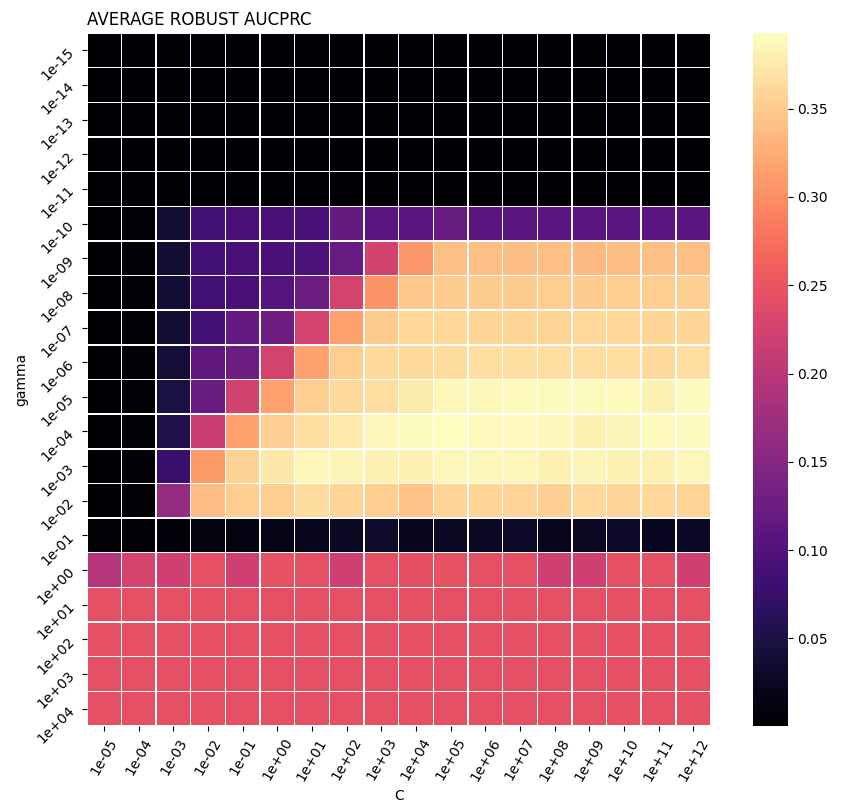
\includegraphics[width=0.7\textwidth]{Kap4/reoptk.png} \\
(a) SVM Lineal & (b) SVM RBF, 100 bins
\end{tabular}
\caption{Resultados de la optimización de hiperparámetros para SVM-Lineal y RBF en el tile b278, incluyendo preprocesamientos.}
\label{fig:reopt_param}
\end{figure}


Utilizando estos nuevos parámetros y preprocesamientos, se volvieron a calcular las curvas de precision-recall para cada par de tiles, que se se pueden ver en la figura \ref{fig:testresultsproc}. 

\begin{figure}[h!]
\begin{center}

\begin{tabular}{ccc}

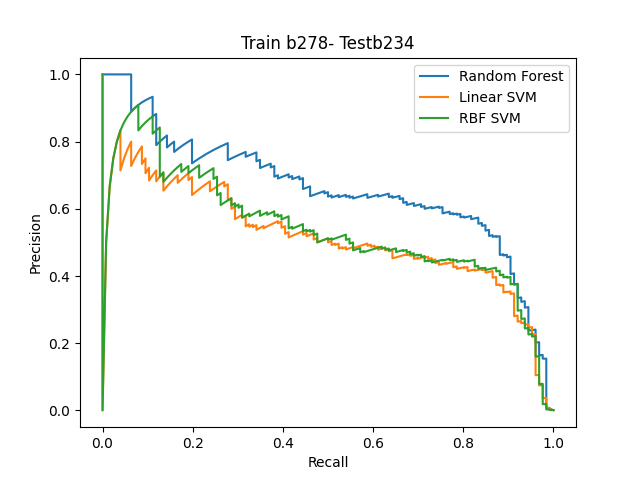
\includegraphics[width=0.32\textwidth]{Kap4/best-train=b278test=b234.png} &
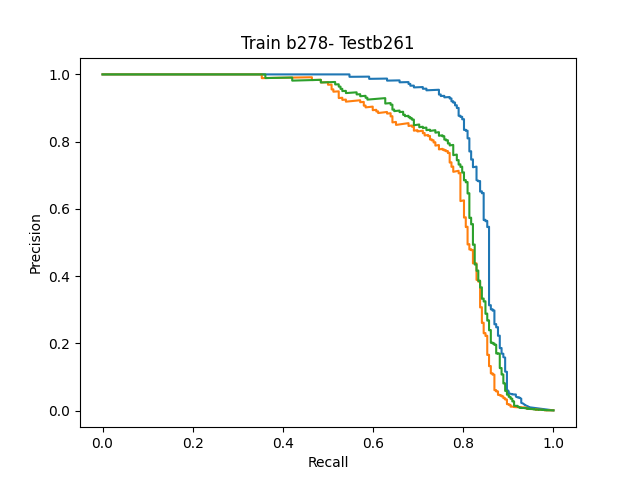
\includegraphics[width=0.32\textwidth]{Kap4/best-train=b278test=b261.png} &
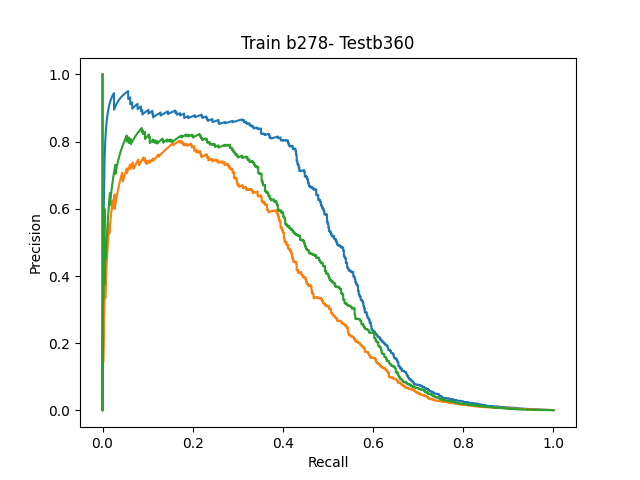
\includegraphics[width=0.32\textwidth]{Kap4/best-train=b278test=b360.png} \\

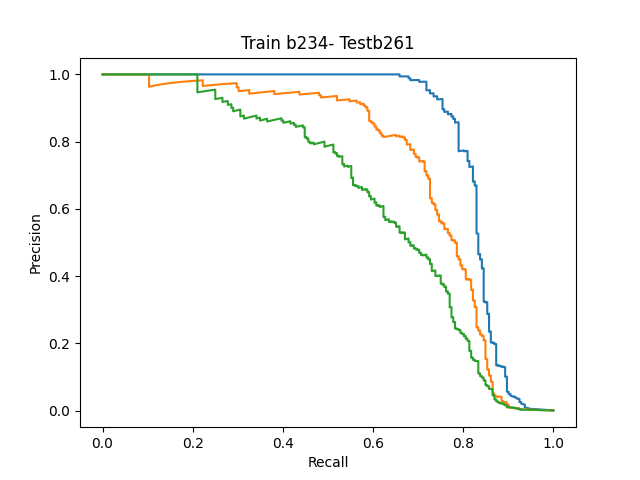
\includegraphics[width=0.32\textwidth]{Kap4/best-train=b234test=b261.png} &
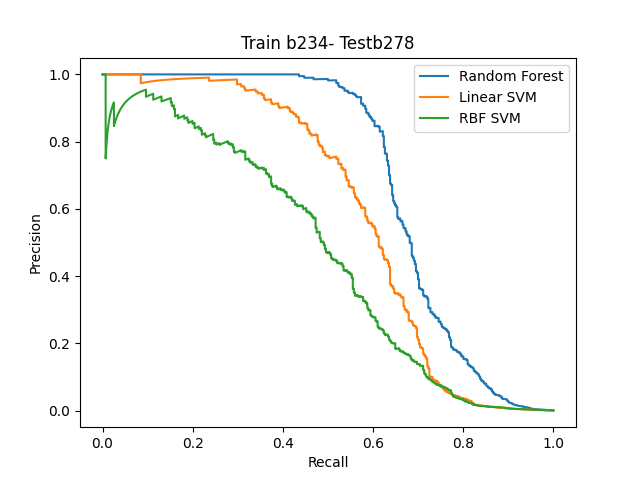
\includegraphics[width=0.32\textwidth]{Kap4/best-train=b234test=b278.png} &
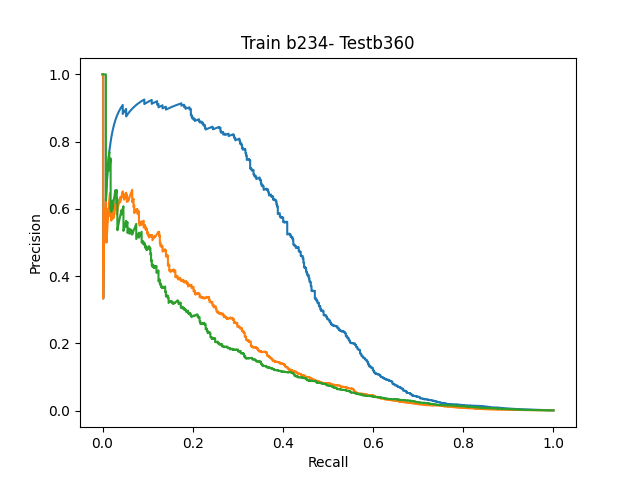
\includegraphics[width=0.32\textwidth]{Kap4/best-train=b234test=b360.png} \\

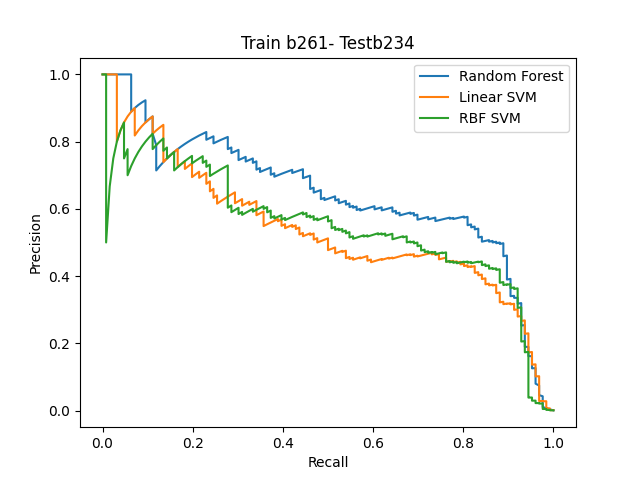
\includegraphics[width=0.32\textwidth]{Kap4/best-train=b261test=b234.png} &
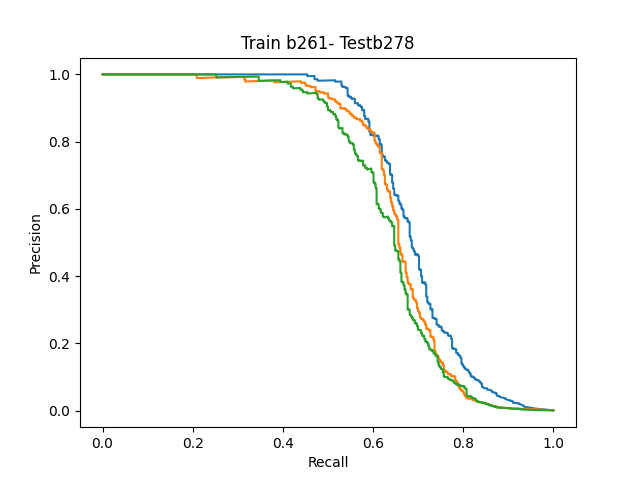
\includegraphics[width=0.32\textwidth]{Kap4/best-train=b261test=b278.png} &
\includegraphics[width=0.32\textwidth]{Kap4/best-train=b261test=b360.png} \\

\includegraphics[width=0.32\textwidth]{Kap4/best-train=b360test=b234.png} &
\includegraphics[width=0.32\textwidth]{Kap4/best-train=b360test=b261.png} &
\includegraphics[width=0.32\textwidth]{Kap4/best-train=b360test=b278.png}

\end{tabular}

\end{center}
\caption[short]{Curvas de precision-recall obtenidas utilizando Random Forest, Support Vector Machine con kernel linal y Support Vector Machine con kernel RBF, incluyendo hiperparámetros optimizados con preprocesamiento incluido.}
\label{fig:testresultsproc}
\end{figure}

\section{Conclusiones}
\label{baseline_preproc}
Las tablas \ref{tab:linear-gain-preproc} y \ref{tab:rbf-gain-preproc} nos permiten medir numéricamente el incremento en R-AUPRC obtenido en las curvas al utilizar preprocesamientos, respecto a las presentadas en capítulos anteriores. Tanto SVM lineal como SVM RBF se ven beneficiados al utilizar binning, siendo SVM lineal el método que muestra un mayor incremento en performance.



\begin{table}[h!]
\centering
\begin{tabular}{|c|c|c|c|c|c|}
\hline
\textbf{Train tile} & \textbf{Test tile} & \textbf{RF} & \textbf{SVM-L} & \textbf{Preproc+SVM-L} & \textbf{Gain}              \\ \hline
b278                & b234               & 0.40        & 0.25           & 0.31                   & 0.06                       \\ \hline
b278                & b261               & 0.54        & 0.44           & 0.48                   & 0.04                       \\ \hline
b278                & b360               & 0.21        & 0.08           & 0.14                   & 0.06                       \\ \hline
b234                & b278               & 0.39        & 0.21           & 0.29                   & 0.09                       \\ \hline
b234                & b261               & 0.53        & 0.37           & 0.44                   & 0.07                       \\ \hline
b234                & b360               & 0.14        & 0.02           & 0.04                   & 0.02                       \\ \hline
b261                & b278               & 0.39        & 0.33           & 0.36                   & 0.02                       \\ \hline
b261                & b234               & 0.39        & 0.25           & 0.30                   & 0.06                       \\ \hline
b261                & b360               & 0.13        & 0.07           & 0.12                   & 0.05                       \\ \hline
b360                & b278               & 0.45        & 0.27           & 0.30                   & 0.04                       \\ \hline
b360                & b234               & 0.42        & 0.20           & 0.26                   & 0.06                       \\ \hline
b360                & b261               & 0.54        & 0.39           & 0.41                   & 0.02                       \\ \hline
\multicolumn{2}{|c|}{avg}                & .38         & .24            & .29                    & {\color[HTML]{009901} .05} \\ \hline
\end{tabular}
\caption{ En esta tabla podemos ver el incremento en R-AUPRC que se obtiene al utilizar preprocesamientos en SVM lineal. }
\label{tab:linear-gain-preproc}
\end{table}

% Please add the following required packages to your document preamble:
% \usepackage[table,xcdraw]{xcolor}
% If you use beamer only pass "xcolor=table" option, i.e. \documentclass[xcolor=table]{beamer}
\begin{table}[h!]
\centering
\begin{tabular}{|c|c|c|c|c|c|}
\hline
\textbf{Train tile} & \textbf{Test tile} & \textbf{RF} & \textbf{SVM-RBF} & \textbf{Preproc+SVM-RBF} & \textbf{Gain}              \\ \hline
b278                & b234               & 0.40        & 0.28             & 0.32                     & 0.04                       \\ \hline
b278                & b261               & 0.54        & 0.49             & 0.50                     & 0.01                       \\ \hline
b278                & b360               & 0.21        & 0.14             & 0.16                     & 0.02                       \\ \hline
b234                & b278               & 0.39        & 0.22             & 0.30                     & 0.09                       \\ \hline
b234                & b261               & 0.53        & 0.41             & 0.45                     & 0.04                       \\ \hline
b234                & b360               & 0.14        & 0.03             & 0.07                     & 0.03                       \\ \hline
b261                & b278               & 0.39        & 0.37             & 0.37                     & 0.00                       \\ \hline
b261                & b234               & 0.39        & 0.30             & 0.33                     & 0.03                       \\ \hline
b261                & b360               & 0.13        & 0.11             & 0.12                     & 0.02                       \\ \hline
b360                & b278               & 0.45        & 0.34             & 0.34                     & 0.00                       \\ \hline
b360                & b234               & 0.42        & 0.27             & 0.30                     & 0.03                       \\ \hline
b360                & b261               & 0.54        & 0.46             & 0.45                     & -0.01                      \\ \hline
\multicolumn{2}{|c|}{avg}                & .38         & .29              & .31                      & {\color[HTML]{009901} .03} \\ \hline
\end{tabular}
\caption{ En esta tabla podemos ver el incremento en R-AUPRC que se obtiene al utilizar preprocesamientos en SVM-RBF. Si bien el aumento es menor al observado en SVM Lineal, se puede observar una mejoría consistente. }
\label{tab:rbf-gain-preproc}
\end{table}